\documentclass[11pt,letterpaper,twoside,english]{article}

\usepackage[margin=1.4in]{geometry} % controls the size of the margins

% Special symbols, etc.
\usepackage{amssymb,amsbsy,latexsym,ytableau}
\usepackage{amsmath}
\usepackage{graphics, subfigure, float} 
\usepackage{cancel}
%\usepackage{todonotes}
% Encoding settings
\usepackage[latin1]{inputenc}
\usepackage[american]{babel}
\usepackage[T1]{fontenc} 
\usepackage{tikz}

\usepackage{titling} % allows posttitle command

% AMS Math packages

\usepackage{amscd,amsthm}

\usepackage{verbatim, comment} % can comment out text 
\usepackage{mdwlist} 

% Graphics
%\usepackage[dvips]{graphicx,epsfig,color}
%\usepackage{subfigure}
%\usepackage{pst-all}
%\usepackage{pstricks-add}
\usepackage{hyperref}  % can only be used with pdflatex - gives hyperlinks
\usepackage{bm} % bold math font
\usepackage{bbm}
\usepackage{todonotes}

\newtheoremstyle{theorem}{1em}{1em}{\slshape}{0pt}{\bfseries}{.}{ }{}
\theoremstyle{theorem}
\newtheorem{theorem}{Theorem}
\newtheorem*{theorem*}{Theorem}
\newtheorem{corollary}[theorem]{Corollary}
\newtheorem{proposition}[theorem]{Proposition}
\newtheorem{lemma}[theorem]{Lemma}
\newtheorem{claim}[theorem]{Claim}
\newtheorem{conjecture}[theorem]{Conjecture}
\newtheorem{definition}[theorem]{Definition}
\newtheorem*{claim*}{Claim}

\theoremstyle{remark}
\newtheorem{remark}{Remark}
\newtheorem*{remark*}{Remark}
\newtheorem{algorithm}{Algorithm}
\newtheorem*{question*}{Question}
\newtheorem{question}{Question}
\newtheorem{example}{Example}

\providecommand{\setN}{\mathbb{N}}
\providecommand{\setZ}{\mathbb{Z}}
\providecommand{\setQ}{\mathbb{Q}}
\providecommand{\setR}{\mathbb{R}}
\providecommand{\E}{\mathrm{E}}
\providecommand{\Pr}{\mathrm{Pr}}
\providecommand{\Var}{\mathrm{Var}}

\tikzset
{
    treenode/.style = {circle, draw=black, align=center, minimum size=1cm},
}

\makeatother

\title{Avoidance in permutations} 

\author{Yajit Jain, Deepak Narayanan, Leon Zhang}

\begin{document}

\maketitle

\section{Introduction}
In this paper we investigate pattern avoidance in finite sequences of natural numbers. We begin with an example: consider the sequences 123 and 1324. Note the order relationships of the elements of 123: we have $1< 2 < 3$. Notice in addition that there is an ordered subsequence of 1324 that follows the same general pattern, namely 124. In this situation we say that the sequence 1324 \emph{does not avoid the pattern 123}. We can also examine the sequence 1432, and observe that none of its subsequences have the same order relationships as 123. We say that 1432 \emph{avoids} 123.

With examples of a four element sequence that avoids 123 and a four element sequence that does not avoid 123, it is natural to ask the question: how many four element sequences avoid 123? And more generally, how many $n$-element sequences avoid 123? If we define $s_n(123)$ to be the number of $n$ element sequences that avoid 123, then the question above is equivalent to identifying the sequence $(s_n(123))_n$. In this paper we consider specific cases of a very general avoidance problem, describing the sequence $(s_n(\sigma))_n$ where $\sigma$ is any permutation of the elements of the set $\{1,2,\cdots, k\}\subset\mathbb{N}$ for some $k$.

In Section \ref{S3} we consider sequences $s_n(\pi)$ when $\pi$ is a permutation on the set $\{1,2,3\}$, and prove that the sequence $s_n(\pi)$ for all such $\pi$ is in fact the sequence of Catalan numbers. In Section \ref{S4} we will consider sequences $s_n(\pi)$ when $\pi$ is a permutation of $\{1,2,3,4\}$. In Section \ref{Tn} we consider a variation of the avoidance problem that considers the problem of avoiding sequences in a subset $T_n$ of the permutations of $n$ elements. Before proceeding, however, we formally introduce the notation that will be used through the rest of this paper. 


\subsection{Notation}

\begin{definition}
The set $S_n$ is the collection of permutations of the set $\{1,2,\cdots, n\}$. 
\end{definition}

\begin{example}
$S_3=\{123,132,213,231,312,321\}$. 
\end{example}

\todo{We never define what a pattern is. Either scrub the paper of mentions or define it here}

\begin{remark}
The notation used to describe the elements of $S_n$ above is `one-line' notation.\todo{Jerison wanted us to define this formally, I think} Thus far we have ignored the fact that $S_n$ has a group structure. When discussing this group structure it is convenient to use a different notation known as `cycle' notation.\todo{Also should define this formally} This alternative notation will be used in Section \ref{S4} and an introduction to cycle notation can be found in Appendix []. 

The notation used to describe the elements of $S_n$ above is `one-line' notation. Thus far we have ignored the fact that $S_n$ has a group structure. When discussing this group structure it is convenient to use a different notation known as `cycle' notation. This alternative notation will be used in Section \ref{S4} and an introduction to cycle notation can be found in Appendix []. 
\end{remark}

\begin{definition}
Two finite sequences of distinct positive integers $a_1,\cdots a_k$ and $b_1,\cdots b_k$ have the same relative order if the $i^\text{th}$ largest entry of each unordered set $\{a_1,\cdots,a_k\}$ and $\{b_1,\cdots, b_k\}$ appears in the same position in $a_1\cdots a_k$ and $b_1\cdots b_k$ for each $1\le i\le k$. 
\end{definition}\todo{I changed this definition... take a look and see if you agree with it}

\begin{remark}
Equivalently, two finite sequences of distinct positive integers have the same relative order if the elements in each position of the sequence satisfy the same set of inequalities.
\end{remark}

\begin{definition}
A finite sequence of distinct positive integers $a_1a_2\cdots a_n$ avoids another finite sequence of distinct positive integers $b_1\cdots b_k$ with $n\ge k$ if no subsequence $a_{i_1}a_{i_2}\cdots a_{i_k}$ of $a_1a_2\cdots a_n$ has its terms in the same relative order as $b_1\cdots b_k$. 
\end{definition}

%\begin{remark}
%Let $S_n$ be the set of permutations of $\{1,\cdots, n\}$. There are two conventions commonly used to write elements of $S_n$. The first is $\emph{one-line}$ notation where permutations in $S_n$ are written explicitly, e.g. 43215 is a permutation of $\{1,2,3,4,5\}$ in $S_5$. 
%The second is \emph{cycle notation}, where a cycle $(a_1\cdots a_n)\in S_n$ with $1\le a_i\le n$ acts on a sequence by sending $a_1\mapsto a_2$, $a_2\mapsto a_3$, $\cdots$, $a_n\mapsto a_1$. For example, the cycle $(14)(23)$ sends $12345$ to $43215$. Unless otherwise stated, we will refer to permutations in one-line notation. 
%\end{remark}

\begin{definition} 
A permutation $\sigma\in S_n$ avoids a permutation $\pi\in S_k$ if the sequence of numbers for the one-line notation for $\sigma$ avoids the sequence of numbers for the one-line notation for $\pi$.
\end{definition}

\begin{definition}
For a permutation $\pi\in S_k$, $s_n(\pi)$ represents the number of permutations in $S_n$ that avoid $\pi$. 
\end{definition}



\section{Flipping and Reversing}

In this section we will identify operations that preserve avoidance. Explicitly, we say that an operator $\mathcal{O}$ preserves avoidance if a permutation $\sigma$ avoids $\pi$ if and only if $\mathcal{O}(\sigma)$ avoids $\mathcal{O}(\pi)$. If $\mathcal{O}$ is an avoidance preserving operator then for any $\sigma\in S_k$, $s_n(\sigma)=s_n(\mathcal{O}(\sigma))$ for all $n$ and $k$. Two such operators that we will identify are the `flipping' and `reversing' operators.  Before discussing these operators, we will introduce generating trees, a tool which we use to study pattern avoidance and particularly to prove the avoidance preserving nature of these operators. 

\subsection{Generating Trees}

The generating tree for the sequence $s_n(\pi)$ is the infinite tree whose vertices are elements of $S_n$ that avoid $\pi$. The first node in the tree is always 1. To construct the tree, we define the children of an arbitrary node. Let $\omega\in S_k$ be a node of the generating tree of $s_n(\pi)$. Then the children of $\omega$ are elements of $S_{k+1}$ that avoid $\pi$ and that can be obtained by inserting the integer $k+1$ between integers in $\omega$. Figure \ref{fig:M1} is an example of the generating tree of $s_n(312)$. 

\begin{figure}[h!]
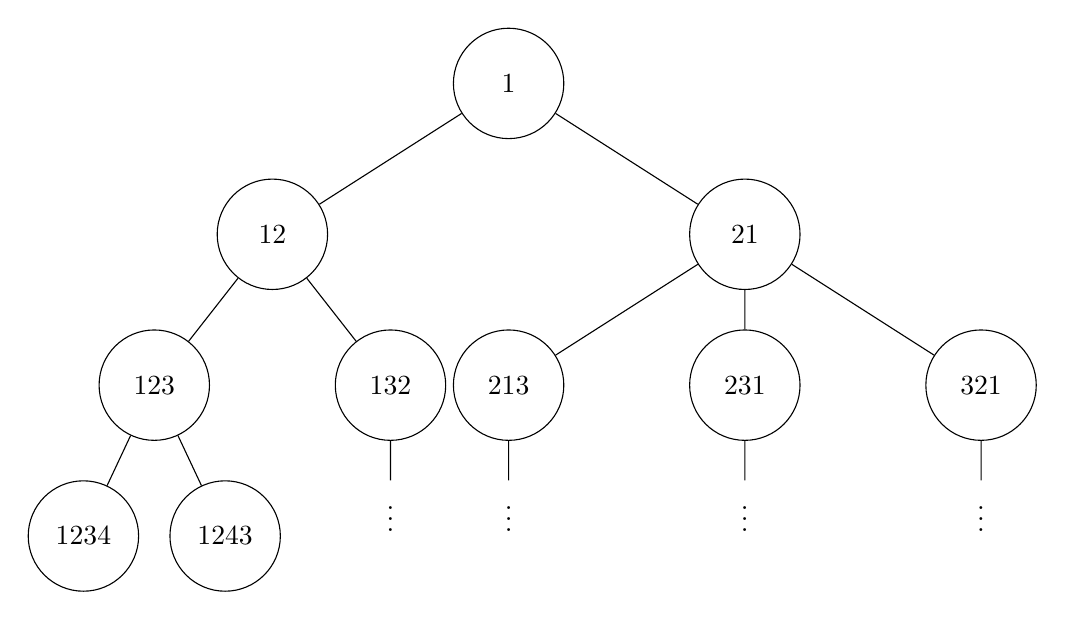
\begin{tikzpicture}[level distance=0.5cm, growth parent anchor={south}, nodes={anchor=north}]
\tikzstyle{hollow node}=[circle,draw,inner sep=0.1mm, text width=1.36cm,align=center]
\tikzstyle{level 1}=[sibling distance=6cm] 
\tikzstyle{level 2}=[sibling distance=3cm] 
\tikzstyle{level 3}=[sibling distance=1.8cm]
\tikzstyle{level 4}=[sibling distance=0.9cm]
\node [hollow node]{1}
	child {
		node[hollow node] {12}
		child{
			node[hollow node]{123}
			child{node[hollow node]{1234}}
			child{node[hollow node]{1243}}
		}
		child{
			node[hollow node]{132}
			child{node{\vdots}}
		}
	}
    	child {
		node[hollow node] {21}
    		child {
			node[hollow node] {213}
			child{node{\vdots}}
		}
      		child {
			node[hollow node] {231}
			child{node{\vdots}}
		}
		child {
			node[hollow node] {321}
			child{node{\vdots}}
		}
    	};

\end{tikzpicture}
\caption{Generating tree of the sequence $s_n(312)$} \label{fig:M1}
\end{figure}

\subsection{Flipping}
In this section we introduce the concept of flipping and use generating trees to prove the `Flipping Lemma.'
\begin{definition}
We define the \emph{flip} of a sequence $a$ as the sequence $b$ with the same elements as $a$, but with the largest element swapped with the smallest element, the second largest element swapped with the second smallest element, etc.  The flipping operator will be denoted by $\mathcal{F}$.  
\end{definition}

\begin{example}
$\mathcal{F}(1324)=4231$.
\end{example}

\begin{lemma}[Flipping Lemma]
The permutation $\sigma$ avoids the permutation $\pi$ if and only if $\mathcal{F}(\sigma)$ avoids $\mathcal{F}(\pi)$. I.e. $\mathcal{F}$ is an avoidance preserving operator. 
\end{lemma}
\begin{proof}
Notice that we only need to proof one direction of this statement. The opposite direction will follow since applying $\mathcal{F}$ twice returns the original permutation. We show that if ${\sigma}$ avoids $\pi$ then $\mathcal{F}(\sigma)$ avoids $\mathcal{F}(\pi)$. Let $\pi=b_1\cdots b_k$. We proceed by induction. Certainly the statement is true for elements of $S_1$. Suppose it is true for elements of $S_{n-1}$. Let $\sigma\in S_n$. If ${\sigma}$ does avoids $\pi$ then $\sigma$ appears in the generating tree of $\pi$.  Then $\sigma=a_1\cdots a_n$ where $a_i\in\{1,\cdots, n\}$. Without loss of generality, let $a_\ell=n$. Then the parent node of $\sigma$ is $\sigma_p=a_1\cdots a_{\ell-1} a_{\ell+1}\cdots a_n$. The induction hypothesis allows us to conclude that $\mathcal{F}(\sigma_p)$ avoids $\mathcal{F}(\pi)$. Now suppose that $\mathcal{F}(\sigma)$ is not a child of $\mathcal{F}(\sigma_p)$. Let $\mathcal{F}(\sigma)=a'_1\cdots a'_{\gamma-1} a_{\gamma}a'_{\gamma+1}\cdots a'_n$ and $\mathcal{F}(\sigma_p)=a'_1\cdots a'_{\gamma-1} a'_{\gamma+1}\cdots a'_n$ with $a'_\gamma=n$. Then $\mathcal{F}(\sigma_p)$ avoids $\pi$ while $\mathcal{F}(\sigma)$ does not. That means that there is a subsequence $\omega$ of $\mathcal{F}(\sigma)$ that has the same relative order as $\mathcal{F}(\pi)$. Let $\mathcal{F}(\pi)= b'_1\cdots b'_k$ with $b'_i=1$ and $b'_j=k$. So $\omega$ contains $a'_\gamma$, and $a'_\gamma$ occupies the same position as $b'_j$. Now if we remove 1 and $n$ from $\mathcal{F}(\sigma)$, then the result does not avoid $\mathcal{F}(\pi)$ with $b'_i=1$ and $b'_j=k$ omitted. Then if we apply a flip, by the induction hypothesis we see that the result of flipping $\mathcal{F}(\sigma)$ with $1$ and $n$ omitted does not avoid $\pi$ with $1$ and $k$ omitted. If we add in 1 and $n$ in the appropriate places to reconstruct $\mathcal{F}(\mathcal{F}(\sigma))=\sigma$ and if we reconstruct $\sigma$ similarly, then $\sigma$ does not avoid $\pi$, a contradiction. 
\end{proof}

\begin{corollary} 
For a permutation $\pi$, $s_n(\pi)=s_n(\mathcal{F}(\pi))$. 
\end{corollary}
\begin{proof}
This result follows because the flipping lemma gives a bijection between permutations that avoid $\pi$ and permutations that avoid $\mathcal{F}(\pi)$. 
\end{proof}
\subsection{Reversing}

\begin{lemma}[Reversing Lemma]
The permutation $\sigma$ avoids the permutation $\pi$ if and only if $\mathcal{R}(\sigma)$ avoids $\mathcal{R}(\pi)$. I.e. $\mathcal{R}$ is an avoidance preserving operator. 
\end{lemma}
\begin{proof}
Again we use the generating tree. Certainly the statement is true for elements of $S_1$. Suppose it is true for elements of $S_{n-1}$. Suppose that $\sigma\in S_n$ avoids $\pi$. Then if $\sigma_p$ is the parent of $\sigma$, $\mathcal{R}(\sigma_p)$ avoids $\mathcal{R}(\pi)$. Now if we add $n$ to the permutation $\mathcal{R}(\sigma_p)$ to construct $\mathcal{F}(\sigma)$, we see that $\mathcal{F}(\sigma)$ must avoid $\mathcal{F}(\pi)$, for if it did not, we could reverse one more time and obtain the result that $\sigma\in S_n$ does not avoid $\pi$, a contradiction. The other direction follows because $\mathcal{R}^2=1$. 
\end{proof}

\begin{corollary} 
For a permutation $\pi$, $s_n(\pi)=s_n(\mathcal{R}(\pi))$. 
\end{corollary}
\begin{proof}
This result follows because the reversing lemma gives a bijection between permutations that avoid $\pi$ and permutations that avoid $\mathcal{F}(\pi)$. 
\end{proof}
\section{Terms in the sequence $s_n(312)$}
\label{S3}

We claim that the sequence of numbers $s_n(312)$ is in fact the sequence of Catalan numbers. Before formally stating and proving the result, however, we prove the following useful lemma.
\begin{lemma}
\label{lemma1}
The permutations of $\{1,2,\dots,k,k+1\}$ ending in $i$ that avoid the pattern $312$ are precisely those of the form,
$$\pi_1 \pi_2 i$$
the concatenation of $\pi_1, \pi_2$, and $i$, where $\pi_1$ is a permutation of $\{1,2,\ldots,i-1\}$ that avoids the pattern $312$ and $\pi_2$ is a permutation of $\{i+1,\ldots,k+1\}$ that avoids the pattern $312$.
\end{lemma}

\begin{proof}

It is easy to see that such a permutation is sufficient for avoiding $312$ and ending in $i$. We will prove that the condition is necessary as well.

First, we define the sets $A=\{1,2,\ldots,i-1\}$ and $B=\{i+1,i+2,\ldots,k+1\}$. For the sake of contradiction, let us assume that there exists some permutation $\pi$ of $\{1,2,...,k,k+1\}$ that ends with value $i$ such that some integer $x < i$ (that is, $x \in A$) is to the right of some integer $y > i$ ($y \in B$). Clearly, this permutation is not of the form described above, and the subsequence $(y, x, i)$ is of the same relative order as 312; as a consequence, $\pi$ does not avoid 312.

It follows that for any permutation $\pi\in S_{k+1}$ avoiding $312$ and ending in $i$, all $x < i$ must be to the left of all $y > i$. Hence $\pi$ must be the concatenation of three subsequences $\pi_1 \pi_2 i$, where $\pi_1$ is a permutation of $\{1, 2, \ldots, i-1\}$ and $\pi_2$ is a permutation of $\{i+1, i+2, \ldots, k+1\}$. Furthermore, it is clear that any subsequences of the permutation $\pi = \pi_1 \pi_2 i$ must avoid $312$ if the entire permutation $\pi$ is to avoid $312$ as well; this implies that the permutations $\pi_1$ and $\pi_2$ must avoid $312$ as well.
\end{proof}

Before we move on to the proof of our main theorem for this section, we look at the sequence of Catalan numbers.

\begin{definition}
The Catalan numbers are the sequence of positive integers $C_i$ defined as follows,
$$C_0=1, \, C_{n+1}=\sum_{i=1}^n C_iC_{n-i} \, \text{for} \; n \geq 0$$
\end{definition}

\begin{theorem}
$s_n(312)$, the total number of permutations of $\{1,2,3,...,n\}$ that avoid the pattern $312$, is equal to $C_n$, the $n^{th}$ Catalan number.
\end{theorem}

\begin{proof}
The inductive hypothesis holds for our base case of $\{1\}$, since the only permutation of $\{1\}$ trivially avoids $312$.

We need to prove the inductive case. Let us first assume that for all $i$ from $1$ to $k$, the number of permutations of $\{1,2,...,i\}$ that avoid the order $312$ as a subsequence is $C_i$.

Now, we want to prove the inductive hypothesis for $\{1,2,...,k,k+1\}$ as well. That is, we want to prove that the number of permutations of $\{1,2,...,k,k+1\}$ that avoid the order $312$ as a subsequence is $C_{k+1}$.

Using our lemma, we count the number of permutations of $\{1,2,...,k,k+1\}$ that avoid $312$ by enumerating through all possible values of the last term of a valid permutation. Consider $\pi$ a permutation of $\{1,2,\ldots, k, k+1\}$ ending in $i$. Let us define the subsets $A$ and $B$ of the  set $\{1,2,...,k+1\} \setminus \{i\}$ as the set of integers less than $i$ and the set of integers greater than $i$ respectively. It is clear from the definition of $A$ and $B$ that $A$ and $B$ are disjoint from each other.

From the above lemma, we know that all permutations of $\{1,2,...,k,k+1\}$ ending in $i$ that avoid $312$ are precisely those of the form
$$\pi = \pi_1 \pi_2 i$$
where $\pi_1$ is a permutation of $A$ that avoids $312$ and $\pi_2$ is a permutation of $B$ that avoids $312$.

It follows that the total number of permutations $\pi$ avoiding $312$ and ending in $i$ is
$$C_{i-1} \cdot C_{k-i+1},$$
since by our induction hypothesis the total number of valid choices for $\pi_1$ is simply $C_{i-1}$, and similarly the total number of valid choices for $\pi_2$ is $C_{k-1+1}$.

Now, summing over all possible values of $i$, we see that the total number of permutations of $\{1,2,...,k+1\}$ that avoid $312$ is equal to,
$$\sum_{i=1}^{k+1} C_{i-1} \cdot C_{k-i+1} = \sum_{i=0}^k C_i \cdot C_{k-i}$$ which is well-known to equal $C_{k+1}$, the $n+1$st Catalan number. The proof  therefore follows by induction.

\end{proof}

It is easy to see that the above proof can be modified slightly to prove that the sequences $s_n(132)$, $s_n(213)$ and $s_n(231)$ are in fact the sequence of catalan numbers as well. In fact, we claim that if $\sigma$ and $\pi$ are both permutations in $S_k$ for some arbitrary $k$, then if $\sigma = flip(\pi)$, $s_n(\pi) = s_n(\sigma)$. This is easy to see since if $a$ is a permutation that avoids $\sigma$, then $flip(a)$ is a permutation that avoids $\pi$ -- since this can be done both ways, it is bijective and we can conclude that the cardinalities of the two sets are equal, or $s_n(\sigma) = s_n(\pi)$.\todo{we should move this up and make it clear from the beginning that this stuff generalizes}

\section{Terms in the sequence $s_n(321)$}

Unfortunately, there is no clear way to reformulate Lemma \ref{lemma1} for the case of avoiding the permutation 321 or 123. As a consequence, the proof in the previous section simply does not hold. Fortunately, however, we still have a closed form expression for $s_n(321)$ (recall that $s_n(321)=s_n(123)$ by our flipping principle). Surprisingly, in fact, the sequence remains the same: $s_n(321)=C_n$, the $n^{th}$ Catalan number. In order to prove this result, we need the machinery of Young tableaux. What follows is a brief exposition of the key results, adapted from Stanley's \emph{Algebraic Combinatorics}.

\begin{definition}
A Young diagram of a partition $\lambda=\{\lambda_1, \lambda_2, \ldots, \lambda_n\}$ of the integer $\sum_{i=1}^n \lambda_i$ is a left-justified array of squares, with $\lambda_i$ squares in the $i$th row.
\end{definition}
\begin{example}
The Young diagram of $(4, 3, 1, 1)$ looks like:
\[
\ytableausetup{centertableaux}
\begin{ytableau}
\ & \ & \ & \ \\
\ & \ & \ \\
\ \\
\
\end{ytableau}
\]
\end{example}

\begin{definition}
A standard Young tableau (or SYT) consists of the Young diagram $D$ of some partition $\lambda$ of an integer $n$, together with the numbers $1, 2, \ldots, n$ inserted into the squares of $D$, so that each number appears exactly once, and every row and column is \emph{increasing}. We call $\lambda$ the \emph{shape} of the SYT.
\end{definition}

\begin{example}
There are five SYT of the shape $(2, 2, 1)$. They are given by
\[\ytableausetup{aligntableaux=top}
\begin{ytableau}
1 & 2 \\
3 & 4\\
5
\end{ytableau}\ \ \ \ \
\hfill
\begin{ytableau}
1 & 2 \\
3 & 5\\
4
\end{ytableau}\ \ \ \ \
\hfill
\begin{ytableau}
1 & 3 \\
2 & 4\\
5
\end{ytableau}\ \ \ \ \
\hfill
\begin{ytableau}
1 & 3 \\
2 & 5\\
4
\end{ytableau}\ \ \ \ \
\hfill
\begin{ytableau}
1 & 4 \\
2 & 5\\
3
\end{ytableau}.\]
\end{example}

\begin{definition}
Let $u$ be a square of the Young diagram of the partition $\lambda$. Then the hook $H(u)$ is the set of all squares directly to the right of $u$ or directly below $u$, including $u$ itself. The size of $H(u)$ is called the hook length of $u$, and is denoted $h(u)$.
\end{definition}

\begin{example}
In the Young diagram of the partition $(4, 2, 2)$ below, each square $u$ contains its hook length $h(u)$.
\[\ytableausetup{centertableaux}
\begin{ytableau}
6 & 5 & 2 & 1\\
3 & 2\\
2 & 1
\end{ytableau}\]
\end{example}

\begin{theorem}
Let $\lambda$ be a partition of $n$. Then $f^\lambda$, the number of SYT of shape $\lambda$, is given by
\[f^\lambda=\frac{n!}{\prod_{u\in \lambda} h(u)},\]
where the notation $u\in \lambda$ means that $u$ ranges over all squares of the Young diagram of $\lambda$.
\end{theorem}

The theorem above is called the \emph{hook-length formula}.

\begin{example}
The diagram above for the hook lengths of $\lambda=(4, 2, 2)$ tells us that the number of SYT of shape $\lambda$ is given by
\[\frac{8!}{6\cdot 5\cdot 2 \cdot 1 \cdot 3 \cdot 2 \cdot 2\cdot 1}=56.\]
\end{example}

It is an easy application of the hook-length formula to prove the following theorem:

\begin{theorem}
The number of SYT of shape $(n, n)$ is given by $C_n$, the $n^{th}$ Catalan number.
\end{theorem}

We need only one more result before we are ready to prove our central result.

\begin{theorem}
There exists an algorithm (called the \emph{RSK algorithm}) which defines a bijection between the set of permutations in $S(n)$ avoiding a decreasing subsequence of length 3 and the set of pairs of size-$n$ SYT of the same shape and at most two rows. 
\end{theorem}\todo{give a citation for this}
Using all this machinery and all these results, we are finally able to prove the closed-form expression for $s_n(321)$.
\begin{theorem}
The total number of permutations of $\{1,2,3,\ldots, n\}$ that avoid the order 321 as a subsequence is $C_n$, where $C_n$ is the $n^{th}$ Catalan number.
\end{theorem}
\begin{proof}
By the first part of Theorem 12, there are $s_n(321)$ elements in the set $A$ of pairs of size-$n$ SYT of the same shape and at most two rows. By Theorem 11, the set $B_n$ of SYT of shape $(n, n)$ has its size given by $C_n$. We will construct a bijection between the sets $A_n$ and $B_n$: because $|A_n|=s_n(321)$ and $|B_n|=C_n$, it will therefore follow that $s_n(321)=C_n$, as desired.

Given any pair of size $n$ Young tableaux of the same shape and at most two parts, take the second tableau and invert its numbers: that is, send $i$ to $2n+1-i$ for all $i$. Now rotate the Young tableau and `fit' it into the first tableau. We demonstrate this process for a pair of Young tableaux with $n=6$: we begin with
\[\ytableausetup{aligntableaux=top}
\begin{ytableau}
1 & 2 &3&4\\
5 & 6
\end{ytableau} \ \ \ \ \ 
\hfill
\begin{ytableau}
1 & 3 & 4 & 5\\
2 & 6
\end{ytableau}.\]
Inverting the numbers of the second tableau gives us
\[\ytableausetup{aligntableaux=top}
\begin{ytableau}
1 & 2 &3&4\\
5 & 6
\end{ytableau} \ \ \ \ \ 
\hfill
\begin{ytableau}
12 & 10 & 9 & 8\\
11 & 7
\end{ytableau}.\]
Finally, rotating the second Young tableau and fitting it into the first gives us
\[\ytableausetup{aligntableaux=top}
\begin{ytableau}
1 & 2 &3&4&7&11\\
5 & 6&8&9&10&12
\end{ytableau},\]
a valid Young tableau of shape $(6, 6)$. 

Beginning with a pair of size $n$ Young tableaux of shape $\lambda$ and at most two parts, it is easy to see that this process always yields a valid Young tableau of shape $(n, n)$. Indeed, we can define its inverse: given any Young tableau for the partition $(n, n)$, we can find the shape formed by all numbers greater than $n$: split it off from the original tableau, rotate it, and invert the numbers to get a pair of size $n$ Young tableau of the same shape and at most two parts. These processes can be easily checked to be inverses: hence the two sets are of the same size, and the proof follows.
\end{proof}

\section{Conjectures on $s_n(\pi)$ for $\pi\in S_4$}
\label{S4}

In this section we present our findings and conjectures about sequences $s_n(\pi)$ for $\pi\in S_4$. We computed values up to $s_{9}$. It appears that there are three sequences that appear, and we have sorted the permutations according to which sequence they produce and paired them with their flips.  

We define the following sequences based on the first nine terms:
$$
A:=1,2,6,23,103,512,2740,15485,91245\ldots
$$
$$
B:=1,2,6,23,103,513,2761,15767,94359\ldots
$$
$$
C:=1,2,6,23,103,513,2762,15793,94776\ldots
$$

The table below lists the elements of $S_4$ generate sequences $A,B,C$ for the first 8 terms.

\begin{center}
\begin{tabular}{|c|c|c|}
B &A&C\\
\hline
1234, 4321&4132, 1423&4231, 1324\\
1243, 4312&4213, 1342&\\
1432, 4123&2431, 3124&\\
2134, 3421&2413, 3142&\\
2143, 3412&2314, 3241&\\
2341, 3214&&\\
\end{tabular}
\end{center}

There is no guarantee that these sequences will not diverge and produce more than three distinct sequences, however for now we hypothesize that $A$, $B$, and $C$ are the only sequences that arise for $s_n(\pi)$ with $\pi\in S_4$. Assuming this hypothesis, if we write each length four permutation in cycle notation, a pattern begins to emerge. 

\begin{center}
\begin{tabular}{|c|c|c|}
B &A&C\\
\hline
(1),(14)(23)&(243),(142)&(23),(14)\\
(34),(1423)&(234),(143)&\\
(24),(1432)&(124),(132)&\\
(12),(1324)&(123),(134)&\\
(12)(34),(13)(24)&(1243),(1342)&\\
(1234),(13)&&\\
\end{tabular}
\end{center}

So we conjecture that sequence $A$ is characterized by elements of $S_4$ that are three cycles or four cycles when written in cycle notation. Sequence $B$ seems to be characterized by either a pair of disjoint two cycles paired with a flip that is a 2-cycle, or a single 4-cycle paired with a flip that is a 2-cycle. Sequence $C$ appears to be characterized by a 2-cycle paired with a 2-cycle as a flip. 


\section{Avoidance of permutations of $T_n$}
\label{Tn}
We now impose further restrictions on the set of permutations $S_n$. This new set of permutations, $T_n$ is defined follows.

\begin{definition}
For even $n$, $T_n$ is defined as the set of all permutations $\sigma \in S_n$ for which $1,3,5,\ldots,2n-1$ appear in increasing order, and $2i$ always appears to the right of $2i-1$.
\end{definition}

Since $T_n$ is only defined for even $n$, henceforth we shall refer to $T_n$ as $T_{2m}$ where $m$ is any integer greater than or equal to $0$.

Given the above definition of $T_{2m}$, we prove the following result about the cardinality of $T_{2m}$.

\begin{theorem}
$|T_{2m}| = 1 \cdot 3 \cdot 5 \cdot \ldots \cdot (2m-1)$
\end{theorem}

\begin{proof}
Observe that since $1,3,5,\ldots,2m-1$ must appear in increasing order in $T_{2m}$, our problem is now reduced to determining the relative order of $2,4,6,\ldots,2m$ with respect to each other, as well as with respect to $1,3,5,\ldots,2m-1$.

Let us first try to insert $2m$ into the sequence $1,3,5,\ldots,2m-1$. Clearly, the way $T_{2m}$ is defined, $2m$ can be inserted into only $1$ slot, the one following $2m-1$. (Here we define a slot as a gap between two existing elements of the sequence, or the gap that follows the last element of the sequence or the gap that precedes the first element of the sequence)

Now, let us try to insert $(2m-2)$ into the sequence. $(2m-2)$ can be inserted into $3$ slots in the sequence -- the one between $2m-3$ and $2m-1$, the one between $2m-1$ and $2m$ or the one following $2m$.

Now, if we try to insert $(2m-4)$ into this incompletely formed sequence, we will see that there are $5$ possible locations into which this number can be inserted. Continuing this for all even numbers upto $2$, we observe that the total number of ways such a sequence can  be created is equal to $1 \cdot 3 \cdot 5 \cdot \ldots \cdot (2m-1)$, as desired.
\end{proof}

Studying avoidance of permutations in $T_n$ seems an interesting exercise. In the following section, we consider the sequence of numbers $t_n(\pi)$, defined as the number of permutations in $T_n$ that avoid the permutation $\pi$. In particular, we consider permutations $\pi \in S_3$.

Before stating our conjectures, we present the computed sequences. Note that since the sequence $T_n$ is defined only for even $n$, we only present the even terms of the sequence $t_n$.

$$t_n(123) = 1, 0, 0, 0, 0, \ldots$$
$$t_n(132) = 1, 1, 1, 1, 1, \ldots$$
$$t_n(213) = 1, 2, 4, 8, 16, \ldots$$
$$t_n(231) = 1, 2, 4, 8, 16, \ldots$$
$$t_n(312) = 1, 3, 12, 55, 273, \ldots$$
$$t_n(321) = 1, 3, 12, 55, 273, \ldots$$

It is easy to see why $t_n(123)$ and $t_n(132)$ behave the way they do -- since all odd numbers in $T_n$ are increasing, it is impossible to have a permutation in $T_n$ that avoids $123$ and the permutation consisting of all increasing integers is the only permutation of $T_n$ that avoids $132$.

More interesting is the equivalences between $213$ and $231$, and $312$ and $321$. We will prove the equivalence between $312$ and $321$ below, but before doing so, we first state and prove the following lemmas which will be useful in our proof.

\begin{lemma}
\label{tn_avoidance}
If $a$ and $b$ are two elements that appear in a permutation in $T_n$ such that $a$ is to the left of $b$, then if $a > b$, $b$ must be even.
\end{lemma}

\begin{proof}
For the sake of contradiction, let us assume that $b$ is odd. Then there exist two possibilities that need to be considered -- one, that $a$ is odd, and two, that $a$ is even.

\begin{itemize}
\item \textbf{Case 1:} $a$ is odd.

Note that all permutations in $T_n$ must have odd elements monotonically increasing. So if $a$ appears to the left of $b$, and both $a$ and $b$ are odd, then $a$ must be less than $b$ -- a contradiction. Hence, we conclude that $a$ can't be odd.

\item \textbf{Case 2:} $a$ is even.

For all permutations $\sigma$ in $T_n$, every even element $j$ must be to the right of all odd elements less than $j$. From this, we conclude that since $a$ is even, it must be to the right of all odd numbers less than it. But $b$ is an odd number less than $a$ -- we conclude that $a$ can't be even either.
\end{itemize}

Since $a$ can't be odd or even if $b$ is odd, we conclude that $b$ must be even, as desired.
\end{proof}

\begin{lemma}
\label{swapping_lemma}
If $x, y, z$ is a three-element subsequence of a permutation $\pi$ in $T_n$ such that $x > y > z$ or $x > z > y$, then swapping $y$ and $z$ in the permutation $\pi$ yields a permutation $\pi'$ that also belongs to $T_n$.
\end{lemma}

\begin{proof}
From Lemma \ref{tn_avoidance} we see that both $y$ and $z$ must be even. Then there exist two cases that need to be covered.
\begin{itemize}
\item \textbf{Case 1:} $x$ is odd.

If $x$ is odd, then it is clear that the permutation $\pi'$ obtained from swapping $y$ and $z$ is still valid, since both $y$ and $z$ are to the right of the odd numbers $y-1$ and $z-1$ (since $y-1$ and $z-1$ are themselves to the left of $x$ since they are strictly less than $x$)

\item \textbf{Case 2:} $x$ is even.

If $x$ is even, then $x-1$ which is an odd number greater than both $y-1$ and $z-1$, must be to the left of $x$. Since $y-1$ and $z-1$ are already to the left of $x-1$, we conclude that swapping $y$ and $z$ still ensures that $y$ and $z$ are both to the right of $y-1$ and $z-1$.
\end{itemize}
Hence, we see that regardless of whether $x$ is even or odd, swapping $y$ and $z$ in a permutation $\pi \in T_n$ if $x > y > z$ or $x > z > y$ yields a permutation $\pi'$ that also belongs to $T_n$.
\end{proof}

Given these lemmas, we now present a proof for $t_n(312) = t_n(321)$.

\begin{theorem}
$t_n(312) = t_n(321)$
\end{theorem}

\begin{proof}
First observe from Lemma \ref{tn_avoidance} that if $x, y, z$ is a subsequence of three elements of a permutation in $T_n$ in the relative order $312$ or $321$, then both $y$ and $z$ must be even.

Before proving that there exists a bijective mapping between the set of permutations in $T_n$ that avoid $312$ (call this set $A$) and the set of permutations in $T_n$ that avoid $321$ (call this set $B$), we establish a chain of transformation moves that can be used to transform an element $a \in A$ to an element $b \in B$.

Consider a permutation $\pi$ in $T_n$ that avoids $312$. For each permutation $\pi \in T_n$ that avoids $312$, we want to show that there exists a sequence of transformation moves that transforms $\pi$ to a unique permutation $\pi'$ that avoids $321$.

If the original permutation $\pi$ avoids $321$ already, then clearly $\pi' = \pi$ avoids $321$.

Now if $\pi$ does not avoid $321$, there must exist some sub-sequence $x, y, z$ in $\pi$ in the relative ordering $321$. From Lemma \ref{swapping_lemma}, we see that swapping $y$ and $z$ in the permutation $\pi$ yields another valid permutation $\pi_1$ in $T_n$ -- note that the permutation produced after this swap has $x, y, z$ in the relative ordering $312$ instead of $321$. Note that $\pi_1$ may still have sub-sequences in the relative ordering $321$, so we may have to perform the above swapping operation again to get some permutation $\pi_2 \in T_n$ such that a sub-sequence $x_1, y_1, z_1$ in $\pi_1$ that has a relative ordering $321$ is in the relative ordering $312$ in $\pi_2$. Continuing this process produces the following chain of permutations,
$$\pi \rightarrow \pi_1 \rightarrow \pi_2 \rightarrow \ldots \rightarrow \pi_k$$
Where the last permutation in the chain $\pi_k$ does not have a single three-element sub-sequence in the relative ordering $321$, that is $\pi' = \pi_k$ is a permutation in $T_n$ that avoids $321$.

This process is completely invertible, since we can take a permutation $\pi'$ in $T_n$ that avoids $321$, and traverse through the above chain in reverse order to obtain a permutation that avoids $312$.

We now prove that there exists a bijection between the sets $A$ and $B$. 

Let $a$ be an arbitrary permutation in $A$. Clearly, by the definition of $A$, $a$ must avoid $312$. Now, we claim that for every element $i$ in the permutation $a$, all even numbers in $a$ to the right of $i$ and less than $i$ must be in decreasing order; if this were not the case, then we would have a subsequence in the relative ordering $312$, which would be a contradiction. It is easy to see that we can make a corresponding claim about permutation $b$, that is for every element $i$ in the permutation $a$, all even numbers in $a$ to the right of $i$ and less than $i$ must be in increasing order.

The above two claims shows there's actually an easy way to transform an arbitrary permutation $a \in A$ to a $b \in B$, and similarly, to transform an arbitrary permutation $b \in B$ to a $a \in A$ -- to obtain a permutation in $B$ from a permutation $a \in A$, for every element $i$ in the permutation $a$, all even elements in $a$ to the right of $i$ less than $i$ should be reversed (that is reordered to in increasing order); similarly to obtain a permutation in $A$ from a permutation $b \in B$, for every element $i$ in the permutation $b$, all even elements in $b$ to the right of $i$, less than $i$ should be reversed (that is reordered to in decreasing order). Since the mapping from $A$ to $B$ is clearly reversible, and hence invertible, we conclude that the mapping we just established between $A$ and $B$ is bijective.

Since there exists a bijective mapping between permutations in $T_n$ that avoid $312$ and permutations in $T_n$ that avoid $321$, we can conclude that $t_n(312) = t_n(321)$.

\end{proof}

Unfortunately, it turns out that proving the equivalence between $231$ and $213$ is not as straightforward as above, however we do prove that both the sequences $(t_n(231))$ and $(t_n(213)$ are equal to the sequence $1, 2, 4, 8, \ldots$, and hence equivalent, below.

\begin{theorem}
$t_n(231) = 1, 2, 4, 8, \ldots$
\end{theorem}

\begin{proof}
Proving the above theorem is equivalent to proving that the $m^{th}$ term of $t_n(231)$ is equal to $2^{m-1}$, or that the number of permutations in $T_{2m}$ that avoid $231$ is equal to $2^{m-1}$.

Consider a permutation $\sigma$ in $T_{2m}$ that avoids $231$. Consider an arbitrary even element $2i$ in $\sigma$. For this element $2i$, define $A$ to be the set of numbers greater than $2i$ and to its left in the permutation $\sigma$. First off, note that the set $A$ cannot contain any even numbers, because if it did, then the permutation $\sigma$ would contain a three-element sub-sequence in the relative ordering $231$ -- if $a$ is an even number in the set $A$, then $(a-1, a, 2i)$ would be a three-element sub-sequence of $\sigma$ in the relative ordering $231$ (Note that $a-1$ must be to the left of $a$ in the permutation $\sigma$ because of the way the set $T_{2m}$ was constructed)

Furthermore, the set $A$ cannot contain any odd elements greater than $2i+1$, because if it did, then again the permutation $\sigma$ would contain a three-element subsequence in the relative ordering $231$ -- if $2j+1 > 2i+1$ is an odd number in $A$, then $(2i+1, 2j+1, 2i)$ is a three-element sub-sequence of $\sigma$ in the relative ordering $231$ Therefore, we conclude that the set $A$ either only contains the element $2i+1$, or is empty.

From this we can conclude that the element $2i$ can be inserted into exactly two valid positions in a permutation of length $2m$ -- at index $2i$ and at index $2i+1$. It follows from the above result that when element $2i$ is at index $2i$, element $2i+1$ is at index $2i+1$ in the permutation, and when element $2i$ is at index $2i+1$, element $2i+1$ is at index $2i$. Note that the element $1$ must always be the first element in the permutation, and the element $2m$ must always be the last element.

Combining all these facts together, we see that the number of permutations $\sigma$ in $T_{2m}$ that avoid $231$ must be equal to $2 \cdot 2 \cdot \ldots \cdot 2 = 2^{m-1}$, since every even element can be inserted in exactly two positions in $\sigma$.

\end{proof}

\begin{theorem}
$t_n(213) = 1, 2, 4, 8, \ldots$
\end{theorem}

\begin{proof}
As before, proving the above theorem is equivalent to proving that the $m^{th}$ term of $t_n(213)$ is equal to $2^{m-1}$, or that the number of permutations in $T_{2m}$ that avoid $213$ is equal to $2^{m-1}$.

First, let us define $A_m$ as the set of all permutations in $T_{2m}$ that avoid $213$. It is easy to see that the $m^{th}$ term of $t_n(213)$ is $|A_m|$.

We now claim that for every permutation $\sigma$ in $A_m$, the numbers $2m-1$ and $2m$ must be consecutive in the permutation $\sigma$. We argue that this must be true by contradiction. If this were not the case, then it is easy to see that the permutation $\sigma$ would have a sub-sequence in the relative ordering $213$ -- let $j$ be an element that's between $2m-1$ and $2m$ in $\sigma$. Clearly, $j < 2m -1 < 2m$ (since every element in $\sigma$ other than $2m$ is less than $2m-1$), which means $(2m - 1, j, 2m)$ are in the relative ordering $213$. We conclude that $2m-1$ and $2m$ must be consecutive in $\sigma$.

Furthermore, we see that we can construct $A_m$ from $A_{m-1}$ by inserting the consecutive elements $2m-1, 2m$ into a permutation $\sigma'$ in $A_{m-1}$. We claim that we get a valid permutation $\sigma$ in $A_m$ from $\sigma'$ only if we insert the consecutive elements $2m-1, 2m$ right after either $2m-3$ or $2m-2$ in $\sigma'$ (which themselves are consecutive in $\sigma'$ from the above claim).

First, note that $2m-1, 2m$ must be inserted to the right of both $2m-3$ and $2m-2$, because of the way $T_{2m}$ is defined. Furthermore, if we insert $2m-1, 2m$ right after some $a$ in $\sigma$ not equal to $2m-3$ or $2m-2$, then we see that the produced permutation $\sigma$ has a three-element sub-sequence in the relative ordering $213$ -- $(2m-2, a, 2m-1)$. Hence we conclude that $2m-1, 2m$ must be inserted to the right of either $2m-3$ or $2m-2$; since we can do this for every permutation $\sigma'$ in $A_{m-1}$, we conclude that $|A_m| = 2|A_{m-1}|$.

Given that $|A_1|$ is trivially equal to $1$, we conclude that $|A_m|$, or the $m^{th}$ term of $t_n(213)$ is indeed equal to $2^{m-1}$, as desired.
\end{proof}

Note that even though we proved that the sequences $t_n(231)$ and $t_n(213)$ are both equivalent, the methods used to prove that each sequence is equal to the sequence $1, 2, 4, 8, \ldots$ are vastly different -- this is an interesting topic of research that we would like to pursue as future work.


\section{Appendix A}

Let $S_n$ be the set of permutations of $\{1,\cdots, n\}$. There are two conventions commonly used to write elements of $S_n$. The first is $\emph{one-line}$ notation where permutations in $S_n$ are written explicitly, e.g. 43215 is a permutation of $\{1,2,3,4,5\}$ in $S_5$. 

The second is \emph{cycle notation}, where a cycle $(a_1\cdots a_n)\in S_n$ with $1\le a_i\le n$ acts on a sequence by sending $a_1\mapsto a_2$, $a_2\mapsto a_3$, $\cdots$, $a_n\mapsto a_1$. For example, the cycle $(14)(23)$ sends $12345$ to $43215$. 


\end{document}